\documentclass[a4paper, oneside]{article}
\raggedbottom

% Pacchetti necessari
\usepackage{amssymb} % Simboli matematici extra
\usepackage{amsmath} % Strumenti matematici extra
\usepackage{amsthm} % Teoremi matematici
\usepackage{tikz} % Pacchetto per disegnare grafici
\usepackage{ulem} % Per sottolineato e altro
\usepackage{nicefrac} % Per frazioni carine
\usepackage{float} % Posizionamento dei float
\usepackage{caption} % Personalizzazione dei titoli dei float
\usepackage{subcaption} % Per sottotitoli dei float
\usepackage{matlab-prettifier} % Per il codice Matlab
\usepackage{hyperref} % Per i link ipertestuali
\usepackage{algpseudocode} % Per scrivere pseudocodice
\usepackage{algorithm} % Per gli algoritmi
\usepackage[T1]{fontenc} % Codifica dei font
\usepackage[utf8]{inputenc} % Codifica dei caratteri
\usepackage[english,italian]{babel} % Imposta la lingua del documento
\usepackage{graphicx} % Per l'inserimento di immagini
\usepackage{lipsum} % Generatore di testo fittizio
\usepackage[a4paper,top=3cm,bottom=3cm,left=3cm,right=3cm]{geometry} % Impostazioni dei margini
\usepackage[fontsize=13pt]{scrextend} % Personalizzazione della dimensione del font
\usepackage{titlesec} % Personalizzazione dei titoli dei capitoli
\usepackage{enumitem} % Elenchi numerati

% Impostazioni per il codice Matlab
\lstdefinestyle{matlabStyle}{
    language=Matlab,
    basicstyle=\ttfamily\small,
    keywordstyle=\color{blue},
    commentstyle=\color{green},
    stringstyle=\color{red},
    breaklines=true,
    showstringspaces=false,
    numbers=left,
    numberstyle=\tiny,
    numbersep=5pt,
    morecomment=[l][\color{magenta}]{\#},
    frame=single
}

% Impostazioni per i titoli dei capitoli
\titleformat{\chapter}[display]
  {\normalfont\huge\bfseries}{\chaptertitlename\ \thechapter}{20pt}{\Huge}
\titlespacing*{\chapter}{0pt}{50pt}{40pt}

% Altri pacchetti utili
\usepackage{changepage} % Per regolare i margini localmente
\usepackage{ifthen} % Per costruzioni condizionali
\usepackage{natbib} % Per la bibliografia
\setcitestyle{numbers} % Imposta lo stile delle citazioni

% Pacchetto per i grafici
\usepackage{pgfplots}
\pgfplotsset{compat=1.17}
\usepackage[export]{adjustbox} % Per l'allineamento delle immagini

\begin{document}

% Inserisce la pagina del frontespizio
\begin{titlepage}
\begin{figure}[!htb]
    \centering
    
\includegraphics[keepaspectratio=true,scale=0.5]{logo.eps}
\end{figure}

\begin{center}
    \LARGE{UNIVERSITÀ DI PISA}
    \vspace{5mm}
    \\ \large{DIPARTIMENTO DI INGEGNERIA DELL'INFORMAZIONE}
    \vspace{5mm}
    \\ \LARGE{Corso di Laurea Triennale in Ingegneria Informatica}
\end{center}

\vspace{15mm}
\begin{center}
    {\LARGE{\bf Rilevamento di curve ad S in immagini satellitari}}
\end{center}
\vspace{30mm}

\begin{minipage}[t]{0.47\textwidth}
	{\large{Relatore:}{\normalsize\vspace{3mm}
	\bf\\ \large{Prof. Marco Cococcioni}}}
\end{minipage}
\hfill
\begin{minipage}[t]{0.47\textwidth}\raggedleft
	{\large{Candidato:}{\normalsize\vspace{2mm} \bf\\\large{Luca Ostinelli\\ }}}
\end{minipage}

\vspace{25mm}
\hrulefill
\\\centering{\large{ANNO ACCADEMICO 2023/2024}}

\end{titlepage}
\thispagestyle{empty} % Non numerare questa pagina
\tableofcontents % Crea l'indice
\newpage

% Spazio tra un paragrafo e l'altro
\setlength{\parskip}{0.5\baselineskip}

% Dedica
%   \cleardoublepage
\thispagestyle{empty}
\vspace*{\stretch{1}}
\begin{flushright}
\itshape 
Ad Asja e Chiara, per la loro vicinanza\\
Ai miei genitori, per il sostegno
\end{flushright}
\vspace{\stretch{2}}
\cleardoublepage

% Inserisce i capitoli
\cleardoublepage
\section{Introduzione alla trasformata di Hough}
La trasformata di Hough è una tecnica utilizzata per rilevare forme geometriche, in particolare linee, cerchi o altri tipi di curve, in un'immagine. Partiamo dal caso più semplice: la trasformata di Hough per linee. Supponiamo di avere un'immagine binaria in cui desideriamo individuare le linee presenti. La trasformata di Hough per linee si basa sull'idea che ogni linea può essere rappresentata da un punto nel parametro spazio. Questo spazio è definito dalle due coordinate $(\rho,\ \theta)$, dove $\rho$ è la distanza dalla linea all'origine e $\theta$ è l'angolo tra la linea e l'asse $x$. \par
Il processo di trasformazione di Hough coinvolge la scansione di ciascun punto nell'immagine binaria. Per ogni punto nero, viene eseguita una scansione attraverso il parametro spazio $(\rho,\ \theta)$. Per ogni valore di $\rho$ e $\theta$, viene incrementato un accumulatore.\par
Una volta completata la scansione, i picchi nell'accumulatore indicano le linee rilevate nell'immagine. Tuttavia, è necessario impostare una soglia critica sull'accumulatore nel caso in cui si voglia selezionare solo i picchi significativi; ad esempio, rette che abbiano uno o più segmenti che insieme siano abbastanza lunghi.\par
La trasformata di Hough per linee è ampiamente utilizzata in applicazioni di visione artificiale ed elaborazione delle immagini, utili in settori come il riconoscimento di forme e oggetti, l'elaborazione di immagini mediche, la visione robotica, il controllo di qualità industriale, la guida autonoma e l'analisi di documenti.\par
La trasformata di Hough è stata introdotta per la prima volta da Richard Duda e Peter Hart nel 1972 \cite{houghtransform}.\par
Nella pagina successiva,  vediamo un semplice \hyperref[lst:houghlineare]{esempio di pseudocodice} per la visualizzazione di tale trasformata lineare in 3 dimensioni.

\subsection{Altri tipi noti: la trasformata per i cerchi}
Nel caso l'obiettivo sia trovare cerchi all'interno di un'immagine, organizziamo lo spazio in questo modo. Ogni pixel dell'immagine viene rappresentato come un punto nello spazio dei parametri Hough, dove i parametri sono le coordinate del centro $(x,\ y)$ e il raggio $r$. Utilizzando un accumulatore tridimensionale, vengono accumulati i voti per ogni possibile centro del cerchio e raggio, consentendo l'individuazione dei cerchi mediante l'identificazione dei picchi nell'accumulatore. \par
Una volta individuati i picchi nell'accumulatore, che rappresentano i centri e i raggi dei cerchi rilevati, è possibile applicare ulteriori criteri di filtraggio, come la soglia o altri criteri di selezione dei picchi, per raffinare la selezione dei cerchi.

\newpage
\lstinputlisting[
    style=matlabStyle,
    caption={Codice MATLAB per la trasformata di Hough lineare},
    label={lst:houghlineare}
]{codici/trasformataDiHoughLineare.m}
\newpage

\subsection{Obiettivo}
L'obiettivo di questo lavoro è sviluppare un approccio innovativo per identificare e tracciare curve a forma di S nelle immagini satellitari. Per raggiungere questo scopo, abbiamo per prima cosa parametrizzato un prototipo di curva ad S, nello specifico una sigmoide, tramite due variabili.\par
Dopodiché, mediante questa parametrizzazione, con la semplice applicazione dei principi standard, siamo arrivati a costruire un tensore\footnote{la nozione di tensore generalizza tutte le strutture definite usualmente in algebra lineare a partire da un singolo spazio vettoriale\cite{wiki:tensore}.} in quattro dimensioni, due che indicassero le coordinate del centro e due per la curva vera e propria, il quale conterrà il numero di occorrenze che tale curva in quel punto ha nell'immagine.\par
Successivamente, abbiamo modificato alcuni principi originali della trasformata per adattarla ad esigenze diverse. Tra i risultati della trasposizione della trasformata di Hough, infatti, c'è il limite abbastanza gravoso della crescita dimensionale.\par
La nostra metodologia, di conseguenza, si distingue perché utilizzeremo una trasformata che converte uno spazio in origine a cinque dimensioni in uno a tre dimensioni, consentendoci di tralasciare dettagli più complessi ma spesso irrilevanti e di gestire più comodamente la visualizzazione del risultato.\par

\subsection{Trasformata generalizzata}
Esiste anche un altro metodo, che enunciamo ma che non tratteremo, di approcciarsi al problema. Questo tralascia l'impostazione analitica per concentrarsi sui modelli di adattamento.\par
Il Generalized Hough Transform (GHT)\cite{ballard1981generalizing}, introdotto da Dana H. Ballard nel 1981, è una modifica della trasformata di Hough che utilizza il principio del riconoscimento dei modelli. Mentre la trasformata di Hough originale era utilizzata per rilevare forme analiticamente definite (come linee, cerchi, ellissi, ecc.), il GHT consente di rilevare oggetti arbitrari descritti tramite un modello. Questa modifica trasforma il problema di individuare un oggetto in un'immagine nel problema di trovare i parametri di trasformazione che mappano il modello nell'immagine.
\cleardoublepage
\section{L'algoritmo di Hough per curve ad S}
\subsection{Parametrizzazione della curva}
Come anticipato nell'introduzione, la prima cosa da fare è determinare quale forma analitica vogliamo andare ad individuare nell'immagine.\par
Prendiamo una sigmoide semplice centrata in $(0,\ 0)$:
$$y(x)=\frac{e^x}{1+e^x}-0.5$$
\begin{center}
\begin{tikzpicture}
\begin{axis}[
    axis lines = middle,
    xlabel = \( x \),
    ylabel = \( y \),
    xmin = -10, xmax = 10,
    ymin = -0.6, ymax = 0.6,
    width = 15cm, height = 6.5cm,
    grid = both,
    grid style = {dashed, gray!50},
    samples = 1000,
    domain = -10:10
]
\addplot[blue, ultra thick] {exp(x)/(1+exp(x))-0.5};
\end{axis}
\end{tikzpicture}
\end{center}

Questa curva si adatta perfettamente alle necessità che abbiamo. Adesso dobbiamo gestirne la velocità con cui passa dall'asintoto inferiore a quello superiore e l'ampiezza, in modo da poter generare tutte le curve di interesse.\par
Il primo parametro lo chiamiamo $a$ ed il secondo $d$, adesso la formula diventa:

$$y(x)=d\cdot\bigg(\frac{e^{a\cdot x}}{1+e^{a\cdot x}}-0.5\bigg)$$
\begin{center}
\begin{tikzpicture}
\begin{axis}[
    axis lines = middle,
    xlabel = \( x \),
    ylabel = \( y \),
    xmin = -15, xmax = 15,
    ymin = -2.1, ymax = 2.1,
    width = 15cm, height = 6.5cm,
    grid = both,
    grid style = {dashed, gray!50},
    samples = 1000,
    domain = -15:15
]
\addplot[blue, ultra thick] {4*(exp(0.3*x)/(1+exp(0.3*x))-0.5)};
\end{axis}
\node[align=center, below] at (current bounding box.south) {Esempio particolare con $a = 0.3$ e $d = 4$};
\end{tikzpicture}
\end{center}

\newpage

\subsection{Trasposizione dell'algoritmo}
L'\hyperref[lst:ostinelli_Tensore4]{algoritmo} a pagina seguente,  genera tutte le curve con parametri $a$ e $d$ in range prestabiliti. Data la complessità computazionale dell'algoritmo può avere senso, dove è concesso, limitare i domini di $a$ e $d$ per generare e quindi testare meno curve. Ad esempio, volessimo solo curve con derivata prima positiva, basterebbe mantenere $a>0$.\par
Una volta generata una curva, che chiameremo $S$, sovrapponiamo, per ogni pixel di riga $c$, e di colonna $b$, la curva sull'immagine in modo che il suo centro coincida con il pixel.\par
A questo punto contiamo le occorrenze dei pixel neri in corrispondenza della curva, questo numero fornisce una misura della presenza della curva di centro $(c,\ b)$.

\subsection{Punti critici di questo approccio}
Il porting dell'algoritmo di Hough ci mette nelle condizioni di avere un tensore di accumulazione in quattro dimensioni. Questo è un problema poiché è molto complicato trovare un modo di rappresentare le cinque dimensioni in un modo comprensibile all'utente.\par
Disegnare un grafico in cinque dimensioni, rappresenta una sfida significativa a causa della complessità aggiuntiva nell'interpretazione visiva di più variabili. Mentre la rappresentazione di dati in due o tre dimensioni è relativamente intuitiva, aggiungere dimensioni comporta un aumento esponenziale della complessità percettiva.\par
La principale difficoltà risiede, quindi, nel trovare un metodo efficace per visualizzare in modo chiaro e comprensibile tutte e cinque le dimensioni simultaneamente. Le tradizionali tecniche di visualizzazione, come grafici a dispersione o grafici a barre, diventano rapidamente inefficienti e ingombranti con un numero così elevato di dimensioni. Altresì, la sovrapposizione di più informazioni sullo stesso grafico può portare a confusione e difficoltà nel distinguere tra i diversi elementi.\par
Un altro aspetto da tenere in considerazione è che, la memorizzazione di grandi quantità di dati in tensori, diventa computazionalmente più complesso man mano che le dimensioni dei dati aumentano. Questo perché l'aumento delle dimensioni comporta una crescita esponenziale del numero totale di elementi nel tensore.\par
Di conseguenza, viene limitata la capacità di elaborare immagini molto risolute, che a parità di dimensioni hanno molti più valori da salvare ed elaborare.

\newpage
\lstinputlisting[
    style=matlabStyle,
    caption={Pseudocodice per la trasformata di Hough per curve ad S},
    label={lst:ostinelli_Tensore4}
]{codici/Ostinelli_Tensore4.m}
\newpage
\cleardoublepage
\section{Proviamo a fissare una dimensione}
Come abbiamo visto in precedenza, l'approccio di Hough prevede un tensore a quattro dimensioni. Per aggirare parzialmente questo problema, possiamo fissare un parametro della curva, come ad esempio $d$ (l'ampiezza), in modo tale da ridurre a tre il numero delle dimensioni del tensore.\par
Come si può osservare nello \hyperref[lst:ostinelli_Tensore3]{pseudocodice} a pagina seguente, questa soluzione è abbastanza semplice da implementare e permette di risolvere alcuni problemi.\par
In primo luogo, risolviamo parzialmente il problema relativo all'impiego di memoria, poiché abbiamo diminuito il numero di dimensioni, quindi abbiamo sensibilmente meno valori da memorizzare.\par
Per quanto riguarda la difficoltà di rendere intelleggibile una struttura del genere, ci sono degli escamotage che permettono la visualizzazione in maniera chiara delle quattro dimensioni, facendo uso dei colori come nell'esempio seguente.

\begin{figure}[h]
    \centering
    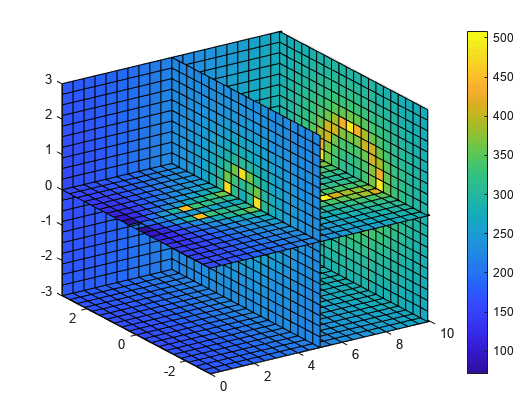
\includegraphics[width=0.8\textwidth]{immagini/altro/volume4D.png}
    \caption{Esempio di Visualizzazione 4D da MathWorks \cite{mathworks}}
\end{figure}

\newpage
\lstinputlisting[
    style=matlabStyle,
    caption={Pseudocodice per la trasformata di Hough per curve ad S con d fissato},
    label={lst:ostinelli_Tensore3}
]{codici/Ostinelli_Tensore3.m}
\newpage

\subsection{Analizziamo qualche esempio}
Come accennato prima, per analizzare gli esempi, usiamo una struttura in cui la quarta dimensione è rappresentata dal colore.\par
Per rendere comprensibile tale struttura usiamo tre piani di taglio, uno per ogni dimensione del tensore, per andare a verificare i colori all'interno della zona d'interesse: $c,\ b$ ed $a$, rappresentati rispettivamente da $y,\ x$ e $z$.\par
Nel \hyperref[fig:4D_ostinelli_1]{primo esempio} è possibile vedere come la curva venga identificata al centro. Dal punto di vista isometrico, notiamo che grazie al parametro $a$, si crea sul piano verticale, una sorta di parabola che identifica la presenza di asintoti abbastanza lunghi.\par
Infatti, nel \hyperref[fig:4D_ostinelli_2]{secondo esempio}, dove la stessa curva ha gli asintoti tagliati, notiamo una parabola sul piano verticale più stretta.\par
Nel \hyperref[fig:4D_ostinelli_3]{terzo} e \hyperref[fig:4D_ostinelli_4]{quarto esempio}, notiamo come sia precisa l'identificazione della posizione del centro della curva. I piani infatti sono stati collocati esattamente nel punto di massimo assoluto del tensore.\par
Nel \hyperref[fig:4D_ostinelli_5]{quinto esempio}, invece, è possibile osservare la maggior larghezza della parabola sull'asse verticale, dovuta all'importante ampiezza della curva stessa. Infatti la curva va a posizionarsi parzialmente su una serie di parametrizzazioni al variare di $a$.\par
Infine, il \hyperref[fig:4D_ostinelli_6]{sesto esempio} verifica la presenza di entrambe le curve singolarmente. Per comodità di lettura, gli assi sono stati posizionati su una delle due sigmoidi. Dopo vedremo che questa precisione sia dovuta al fatto che il parametro $d$ sia fissato.


\foreach \i in {1,...,6} {
    \newpage
    \subsubsection{Esempio in 4 dimensioni n.\i}
    \vfill
    \begin{center}
    \begin{figure}[H]
        \label{fig:4D_ostinelli_\i}
        \centering
        \begin{subfigure}{0.40\textwidth}
            \centering
            \includegraphics[width=\linewidth, frame]{immagini/sintetiche/\i.png}
            \caption*{Input}
        \end{subfigure}

        \vspace{20pt}
        
        \begin{subfigure}{0.43\textwidth}
                \centering
                \includegraphics[width=\linewidth, frame]{immagini/4D_risultati_sintetiche/\i_isometrica.png}
                \caption*{Isometrica}
            \end{subfigure}
            
        \vspace{20pt}
        
        \begin{subfigure}{0.43\textwidth}
                \centering
                \includegraphics[width=\linewidth, frame]{immagini/4D_risultati_sintetiche/\i_sotto.png}
                \caption*{Sotto}
            \end{subfigure}
    \end{figure}
    \end{center}
}

\cleardoublepage
\section{Un approccio diverso}
Il nostro approccio si basa, come l'originale, sul trovare tutte le curve nei range di parametri prestabiliti per ogni pixel dell'immagine.\par
Quindi, a differenza del metodo visto prima, non andiamo a limitare la ricerca delle curve in qualche dimensione. Tuttavia cerchiamo di dimostrare come, nella maggior parte dei casi, sia più sensato identificare le curve in base alla posizione del loro centro rispetto agli altri due parametri.\par
Questo lo facciamo utilizzando una matrice di coordinate $(c,\ b)$ in cui salviamo le informazioni relative ai parametri $(a \text{ e } d)$ ed il numero di occorrenze che tale curva, la migliore, ha nel punto.\par
Com'è possibile osservare nello \hyperref[lst:ostinelli]{pseudocodice} a pagina seguente, alla riga 31 e seguenti, i dati (parametri della curva e occorrenze) vengono salvati solo nel caso in cui non ci sia stata una curva, precedentemente testata, che ha fatto un risultato migliore in termini di occorrenze in quel punto.\par
Questo ridurre le dimensioni del tensore a due (le coordinate del pixel) ci permette, oltre il notevole risparmio di spazio all'interno della memoria, di rappresentare il risultato della trasformata all'interno di un grafico tridimensionale, esattamente come nella trasformata lineare.\par
Gli assi del grafico sono $x$ e $y$ per le coordinate dei pixel e $z$ per le occorrenze.\par
Per un umano è estremamente intuitivo, a questo punto, identificare il centro della curva. Anche il sistema però è in grado, con uno sforzo computazionale ridotto, di trovare il massimo locale.\par
Rimane il problema della soglia critica, da scegliere in base al tipo di applicazione che vogliamo fare dell'algoritmo, che è intrinseco a questo tipo di trasformate.\par
Nella prossima sezione, analizzeremo qualche esempio. Per ognuno di questo abbiamo a disposizione quattro visualizzazioni che riescono a rendere un'idea del grafico tridimensionale:
\begin{enumerate}[itemsep=0pt, topsep=0pt]
    \item una isometrica, che permette di vedere il picco tridimensionale;
    \item una da sotto, utile grazie al colore, per vedere il centro della curva;
    \item vista dall'asse $X$;
    \item vista dall'asse $Y$.
\end{enumerate}

\newpage
\lstinputlisting[
    style=matlabStyle,
    caption={Pseudocodice per la trasformata in 2+1 dimensioni},
    label={lst:ostinelli}
]{codici/Ostinelli.m}
\newpage

\subsection{Analisi degli esempi}
Nel \hyperref[fig:sintentica_ostinelli_1]{primo esempio}, vediamo un picco al centro del grafico che segnala la presenza del centro della curva. Nella visione dall'asse $x$, è possibile notare come ci siano due pendii ai lati del picco.\par
Questo è dovuto alla lunghezza degli asintoti: alcune delle curve centrate nello stesso punto e con parametro $d$ (ampiezza) identico ma con parametro della curva $a$ diverso avranno in comune quella serie di punti.\par
Di conseguenza, la stessa curva, presente nel \hyperref[fig:sintentica_ostinelli_2]{secondo esempio}, che tuttavia ha gli asintoti tagliati, avrà un picco maggiormente isolato senza lasciarsi la scia sui versanti.\par
Nel \hyperref[fig:sintentica_ostinelli_3]{terzo} e \hyperref[fig:sintentica_ostinelli_4]{quarto esempio}, è possibile notare come sia precisa la posizione di identificazione. Con una forma, apprezzabile dalle visualizzazioni ortogonali agli assi $x$ ed $y$, molto simile a quello del \hyperref[fig:sintentica_ostinelli_2]{secondo esempio}.\par
Il \hyperref[fig:sintentica_ostinelli_5]{quinto esempio} dimostra come, in questo tipo di trasformata, dove i parametri della curva vanno in secondo piano rispetto alla presenza o meno della stessa, la sigmoide presente viene segnalata ma non è apprezzabile una significativa differenza per la parte inerente ai parametri $a$ e $d$.\par
Un caso decisamente interessante è il \hyperref[fig:sintentica_ostinelli_6]{sesto esempio} che, grazie alla presenza di due curve, palesa un fatto interessante.\par
I picchi dei relativi centri sono assolutamente ben visibili, di conseguenza ben individuabili anche grazie ad una soglia critica impostabile.\par
Da notare qualche picco più piccolo, ben visibile dall'asse $x$, anomalo. Questo è dovuto alla presenza, nello stesso grafico, di tutti i test delle possibili curve di parametri $a$ e $d$. Di conseguenza, vengono generate curve che intersecano le due presenti nell'immagine come si vede nell'\hyperref[fig:sovrapposizione]{immagine sotto}.\par
Infatti, la curva tratteggiata, potrebbe non essere presente ma essere rilevata in quanto alcuni punti andranno a votare proprio per quella.

\begin{figure}[h]
    \label{fig:sovrapposizione}
    \centering
    \fbox{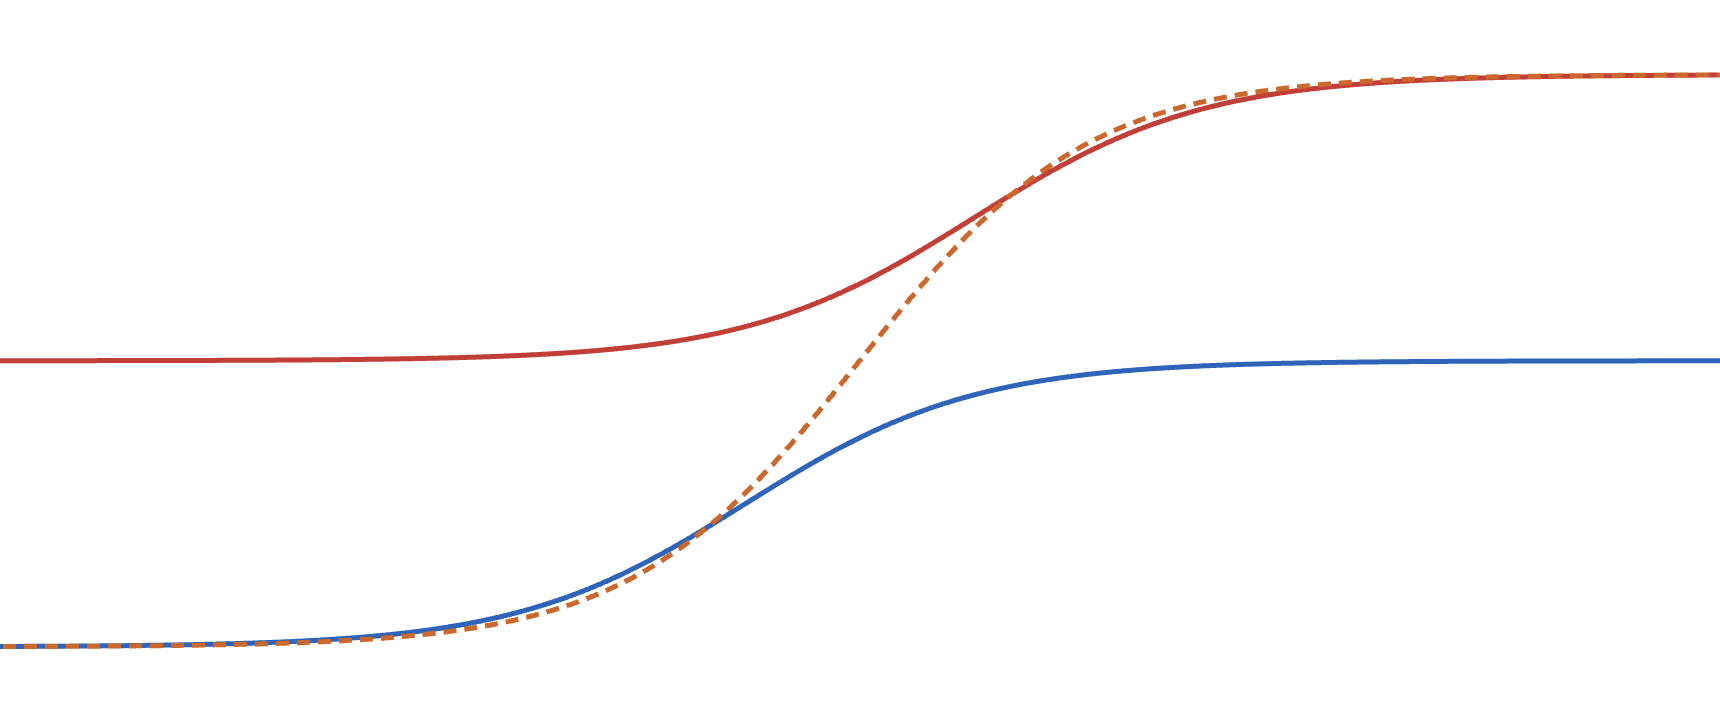
\includegraphics[width=0.71\textwidth]{immagini/altro/sovrapposizione.png}}
    \caption{Esempio di curve sovrapposte con parametro $d$ differente}
\end{figure}


% Esempi
\foreach \i in {1,...,6} {
    \newpage
    \subsubsection{Esempio in 3 dimensioni n.\i}
    \vfill
    \begin{center}
    \begin{figure}[H]
        \label{fig:sintentica_ostinelli_\i}
        \centering
        \begin{subfigure}{0.40\textwidth}
            \centering
            \includegraphics[width=\linewidth, frame]{immagini/sintetiche/\i.png}
            \caption*{Input}
        \end{subfigure}

        \vspace{20pt}
        
        \foreach \j/\desc in {isometrica/Isometrica,sotto/Sotto} {
            \begin{subfigure}{0.38\textwidth}
                \centering
                \includegraphics[width=\linewidth, frame]{immagini/ostinelli_risultati_sintetiche/\i_\j.png}
                \caption*{\desc}
            \end{subfigure}
            \ifnum\pdfstrcmp{\j}{sotto}=0
            \else
                \hspace{20pt}
            \fi
        }

        \vspace{20pt}
        
        \foreach \j/\desc in {davanti_X/Vista da X,davanti_Y/Vista da Y} {
            \begin{subfigure}{0.38\textwidth}
                \centering
                \includegraphics[width=\linewidth, frame]{immagini/ostinelli_risultati_sintetiche/\i_\j.png}
                \caption*{\desc}
            \end{subfigure}
            \ifnum\pdfstrcmp{\j}{davanti_Y}=0
            \else
                \hspace{20pt}
            \fi
        }
    \end{figure}
    \end{center}
}

\cleardoublepage
\section{Proviamo con delle immagini satellitari}
Le immagini satellitari sono realizzate utilizzando sensori in orbita attorno alla Terra. Questi sensori catturano la luce riflessa dalla superficie terrestre in diverse bande dello spettro elettromagnetico.\par
Le curve ad S segnalano la presenza di un target, ma oltre a quel segnale abbiamo un notevole rumore sottoforma di bande verticali multicolore che possono essere il risultato di riflessi atmosferici, errori di calibrazione o disturbi durante la trasmissione dei dati.

\subsection{Eliminazione del rumore}
Prima di applicare \hyperref[lst:ostinelli]{l'algoritmo per la generazione di grafici tridimensionali}, è cruciale affrontare l'aspetto relativo all'elaborazione dell'immagine satellitare, che come detto prima presenta anche la complessità di separare il segnale dal rumore.\par
Per far ciò, è indispensabile sviluppare un metodo efficace per gestire questo tipo di input. Negli esempi a nostra disposizione, siamo riusciti a svolgere un discreto lavoro di separazione delle due componenti tramite un semplice filtro composto da una maschera che seleziona i toni del rosso, eliminando gli altri. Spesso potrebbe essere necessario un procedimento più complesso.

\vspace{10pt}
\lstinputlisting[
    style=matlabStyle,
    caption={Codice per l'isolamento della scala cromatica d'interesse},
    label={lst:PulisciImmagine}
]{codici/PulisciImmagine.m}
\vspace{10pt}

A questo punto, l'immagine ottenuta può essere passata allo \hyperref[lst:ostinelli]{stesso algoritmo} di prima per ottenere la matrice delle occorrenze da graficare.\par
Negli esempi sottostanti, è possibile vedere anche l'esito dell'applicazione di questo filtro.

\newpage
\subsection{Analisi degli esempi reali}
Come vediamo dagli esempi, l'algoritmo è in grado di rilevare correttamente il \hyperref[fig:reale_ostinelli_1]{primo caso}, che è segnalato da un picco proprio in concomitanza del centro della curva.\par
Per quanto riguarda il \hyperref[fig:reale_ostinelli_2]{secondo caso}, invece, abbiamo più considerazioni da fare.\par
Proprio quest'ultimo, infatti, sottopone ad un notevole stress il nostro algoritmo poiché ha una serie di curve, con parametro $a$, che ricordiamo essere la velocità di crescita, molto vario e un parametro $d$, l'ampiezza della curva, pressoché fissa.\par
Il riconoscimento evidenzia infatti un picco in posizione della curva di maggior lunghezza, appartenente alla curva col maggior numero di occorrenze ed una serie di picchi più piccoli in posizione delle altre. Inoltre l'immagine ha delle curve che sono presenti a tratti, proprio in questi casi la scelta della soglia critica ha bisogno di particolari valutazioni, in quanto è autoevidente che tali curve avranno picchi mutiliati.\par
Il problema che avevamo riscontrato parzialemente nel \hyperref[fig:sintentica_ostinelli_6]{sesto esempio} del capitolo precedente\footnote{quello inerente a curve distinte che, per alcuni parametri $a$ e $d$, potrebbero andare a votare per un'unico punto.}, invece, è qui di nuovo presente. Alcune interazioni tra le curve tendono a presentare picchi di minor entità.\par
In immagini reali molto complesse, il nostro algoritmo potrebbe quindi presentare dei falsi positivi difficili da rimuovere.

% Esempi
\foreach \i in {1,...,2} {
    \newpage
    \subsubsection{Esempio con immagine reale n.\i}
    \begin{center}
    \begin{figure}[H]
        \label{fig:reale_ostinelli_\i}
        \centering
        \foreach \j/\desc in {input/Input,modificato/Input modificato} {
            \begin{subfigure}{0.38\textwidth}
                \centering
                \includegraphics[width=\linewidth, frame]{immagini/reali/\i_\j.png}
                \caption*{\desc}
            \end{subfigure}
            \ifnum\pdfstrcmp{\j}{modificato}=0
            \else
                \hspace{20pt}
            \fi
        }

        \vspace{20pt}
        
        \foreach \j/\desc in {isometrica/Isometrica,sotto/Sotto} {
            \begin{subfigure}{0.38\textwidth}
                \centering
                \includegraphics[width=\linewidth, frame]{immagini/ostinelli_risultati_reali/\i_\j.png}
                \caption*{\desc}
            \end{subfigure}
            \ifnum\pdfstrcmp{\j}{sotto}=0
            \else
                \hspace{20pt}
            \fi
        }

        \vspace{20pt}
        
        \foreach \j/\desc in {davanti_X/Vista da X,davanti_Y/Vista da Y} {
            \begin{subfigure}{0.38\textwidth}
                \centering
                \includegraphics[width=\linewidth, frame]{immagini/ostinelli_risultati_reali/\i_\j.png}
                \caption*{\desc}
            \end{subfigure}
            \ifnum\pdfstrcmp{\j}{davanti_Y}=0
            \else
                \hspace{20pt}
            \fi
        }
    \end{figure}
    \end{center}
}
\cleardoublepage
\section{Conclusioni}
Nei capitoli precedenti, attraverso gli esempi osservati, abbiamo approcciato lo stesso problema in diversi modi, utilizzando più di un metodo per migliorare la fruizione all'utente e lo sforzo mnemonico del sistema.\par

\subsection{Approccio classico}\label{conclusioni_caso1}
Applicare direttamente tutti i principi dell'algoritmo di Hough, abbiamo visto essere inefficace agli obiettivi che ci siamo posti. Questo perché l'algoritmo originale prevede di avere una dimensione per ogni parametro della curva nell'immagine; ciò porta ad utilizzare un tensore quadridimensionale.\par
La rappresentazione di cinque dimensioni in modo comprensibile all'utente, cioè che non induca in errori di interpretazione, è pressoché impossibile.\par
Oltre questo, mantenere in memoria una quantità di dati abnorme e, su questi, ricercare massimi locali all'interno del tensore è anche computazionalmente complesso.\par
È di facile comprensione la grande quantità di valori presenti, nel caso si intenda analizzare un'immagine Full-HD\footnote{Le immagini Full HD hanno una risoluzione pari a 1920x1080 pixel.} per un discreto numero di curve. Se ipotiziamo valori di $a$ in un range $[0.1,\ 2]$ con passo di $0.05$ e, $d$ in un range $[10,\ \text{<numero di righe>}]$ con passo $2$, otteniamo facilmente:
$$\text{Numero di valori} = \underbrace{1920\times 1080}_{\text{dim. immagine}}\times\underbrace{\frac{2-0.1}{0.05}}_{\text{valori di a}}\times\underbrace{\frac{1080-10}{2}}_{\text{valori di d}}\approx 20\times10^9$$

\subsection{Approccio classico limitato}\label{conclusioni_caso2}
Successivamente abbiamo provato ad arginare questi due macro problemi fissando una dimensione. Abbiamo deciso di fissare $d$, in quanto è possibile che l'ampiezza delle curve sia dovuta ad una costante fisica: nel caso di satelliti non geostazionari, potrebbe essere la velocità relativa del satellite rispetto alla terra.\par
Per quanto riguarda il numero di valori, questo approccio permette di limitarli relativamente.\par
Nell'esempio di prima, possiamo togliere l'ultimo rapporto, lasciando:
$$\text{Numero di valori} = \underbrace{1920\times 1080}_{\text{dim. immagine}}\times\underbrace{\frac{2-0.10}{0.05}}_{\text{valori di a}}\times \underbrace{1}_{\text{valori di d}}\approx 37\times10^6$$
Questo metodo, a differenza degli altri due, riduce anche le iterazioni necessarie per il computo delle occorrenze.\par
Mentre per quanto riguarda la visualizzazione, abbiamo trovato un metodo che, oltre alle tre dimensioni classiche, usa i colori.\par
Tuttavia, questo metodo crea un grafico che non è esattamente di immediata lettura e questo può portare a notevoli errori. Per avere un'informativa completa è necessario traslare i vari piani di taglio per visualizzare tutte le possibili combinazioni, questo richiede tempo e conoscenza da parte dell'utente.\par

\subsection{Approccio innovativo}
Il nostro approccio coniuga la semplicità rappresentativa del risultato con una ridotta necessità di memoria.\par
Questo perché la struttura che accoglie i dati è una semplice matrice bidimensionale. Essa è rappresentante dell'immagine, quindi abbiamo come coordinate della matrice quelle dei pixel.\par
Come abbiamo visto nell'\hyperref[lst:ostinelli]{algoritmo}, il sistema salva i dati inerenti alla curva testata e al numero di occorrenze che questa ha generato, solo nel caso in cui non ci sia stata una curva già testata con maggior numero di occorrenze.\par
Facendo questo, ci accorgiamo che il numero di dati salvati è leggermente minore del \hyperref[conclusioni_caso2]{secondo caso} e sensibilmente del \hyperref[conclusioni_caso1]{primo}.
$$\text{Numero di valori} = \underbrace{1920\times 1080}_{\text{dim. immagine}}\times\underbrace{3}_{\text{num. parametri}}\approx 6\times10^6$$

\subsubsection{Fragilità principale}
Come abbiamo visto nel \hyperref[fig:sintentica_ostinelli_6]{sesto esempio} delle immagini sintetiche e nel \hyperref[fig:reale_ostinelli_2]{secondo esempio} delle immagini reali, il nostro algoritmo, in caso di più curve ad S presenti nell'immagine, rischia di segnalare la presenza di curve in realtà inesistenti. Questi falsi positivi, sono dati dalla sovrapposizione immaginaria di una curva più grande con le due più piccole.\par
Questo problema è intrinseco alla nostra scelta di rappresentare in uno stesso grafico a prescindere dai parametri delle stesse.

\newpage
\nocite{*} % Cita tutte le voci della bibliografia
\bibliographystyle{unsrtnat} % Stile della bibliografia
\bibliography{bibliografia} % File della bibliografia

% Ringraziamento
%   \cleardoublepage
%   \thispagestyle{empty}

\begin{center}
\textbf{\LARGE Ringraziamenti}
\end{center}

In primo luogo, desidero ringraziare il mio relatore, il Prof. Marco Cococcioni, per il sostegno durante il periodo di sviluppo. I suoi consigli e suggerimenti hanno contribuito in modo significativo a questo lavoro.\par
Un ringraziamento speciale va anche ai miei genitori e tutta la mia famiglia per il loro costante sostegno. Senza di loro, questo risultato non sarebbe stato possibile.\par
Infine, vorrei ringraziare tutti i miei amici storici Asja, Chiara, Iacopo, Alice e quelli incontrati durante questo percorso Simone e Giacomo per essermi stati vicini.\par
Per ultimo a Gianluca, che ha trovato parole di stima per il titolo da conseguito.

\end{document}
